% ****************************************************************************************** % Dissertation template and document class for Princeton University
% Author  : Jeffrey Scott Dwoskin <jdwoskin@princeton.edu>
% Adapted from: http://www.math.princeton.edu/graduate/tex/puthesis.html
% ****************************************************************************************** %


%%% For print copies
%% set 'singlespace' option to set entire thesis to single space, and define "\printmode" to remove all hyperlinks for printed copies of the thesis. Delete all output files before changing this mode -- it will turn hyperref package on and off
%\documentclass[12pt,lot, lof, singlespace]{puthesis}
%\newcommand{\printmode}{}

%%% For the electronic copy, use doublespacing, define "\proquestmode" to use outlined links, instead of colored links. 
\documentclass[12pt,lot, lof]{puthesis}
\newcommand{\proquestmode}{}
% I prefer proquestmode to be off for electronic copies for normal use, since the colored links are less distracting. However when printed in black and white, the colored links are difficult to read. 

%%% For early drafts without some of the frontmatter
% Also see the "ifodd" command below to disable more frontmatter
%\documentclass[12pt]{puthesis}

%%%%%%%%%%%%%%%%%%%%%%%%%%%%%%%%%%%%%%%%%%%%%%%%%%%%%%%%%%%%%\
%%%% Author & title page info

%%%%%%%%%%%%%%%%%%%%%%%%%%%%%%%%
\usepackage{color}
\usepackage{booktabs}

\usepackage{color}
\usepackage{url}

\usepackage{amsmath,amsthm,amssymb}
\usepackage{algorithm,algpseudocode}
\usepackage{enumerate}
\usepackage{multirow}
\usepackage{dirtytalk}
\usepackage{balance}

\newcommand{\mahyar}[1]{\textcolor{blue}{{#1}}}

%%%%%%%%%%%%%%%%%%%%%%%%











\title{ Comparative Analysis between Micro and Macro Agent Evacuation Using PedSim Simulator   }

\submitted{March 2019}  % degree conferral date (January, April, June, September, or November)
\copyrightyear{2019}  % year in which the copyright is secured by publication of the dissertation.
\author{Hrishikesh Narayanankutty}
\adviser{Professor Henry Muccini}  %replace with the full name of your adviser
%\departmentprefix{Program in}  % defaults to "Department of", but programs need to change this.
\department{Informatics}

%%%%%%%%%%%%%%%%%%%%%%%%%%%%%%%%%%%%%%%%%%%%%%%%%%%%%%%%%%%%%\
%%%% Tweak float placements
% From: http://mintaka.sdsu.edu/GF/bibliog/latex/floats.html "Controlling LaTeX Floats"
% and based on: http://www.tex.ac.uk/cgi-bin/texfaq2html?label=floats
% LaTeX defaults listed at: http://people.cs.uu.nl/piet/floats/node1.html

% Alter some LaTeX defaults for better treatment of figures:
    % See p.105 of "TeX Unbound" for suggested values.
    % See pp. 199-200 of Lamport's "LaTeX" book for details.
    %   General parameters, for ALL pages:
    \renewcommand{\topfraction}{0.85}   % max fraction of floats at top
    \renewcommand{\bottomfraction}{0.6} % max fraction of floats at bottom
    %   Parameters for TEXT pages (not float pages):
    \setcounter{topnumber}{2}
    \setcounter{bottomnumber}{2}
    \setcounter{totalnumber}{4}     % 2 may work better
    \setcounter{dbltopnumber}{2}    % for 2-column pages
    \renewcommand{\dbltopfraction}{0.66}    % fit big float above 2-col. text
    \renewcommand{\textfraction}{0.15}  % allow minimal text w. figs
    %   Parameters for FLOAT pages (not text pages):
    \renewcommand{\floatpagefraction}{0.66} % require fuller float pages
    % N.B.: floatpagefraction MUST be less than topfraction !!
    \renewcommand{\dblfloatpagefraction}{0.66}  % require fuller float pages

% The documentclass already sets parameters to make a high penalty for widows and orphans. 

%%%%%%%%%%%%%%%%%%%%%%%%%%%%%%%%%%%%%%%%%%%%%%%%%%%%%%%%%%%%%\
%%%% Use packages

%\usepackage{amsfonts}

%%% For figures
\usepackage{graphicx}
%\usepackage{subfig,rotate}

%%% for comments
\usepackage{verbatim}

%%% For tables
\usepackage{multirow}
% Longtable lets you have tables that span multiple pages.
\usepackage{longtable}

% Booktabs produces far nicer tables than the standard LaTeX tables.
%   see: http://en.wikibooks.org/wiki/LaTeX/Tables
\usepackage{booktabs}

%set parameters for longtable:
% default caption width is 4in for longtable, but wider for normal tables
\setlength{\LTcapwidth}{\textwidth}



%%%%%%%%%%%%%%%%%%%%%%%%%%%%%%%%%%%%%%%%%%%%%%%%%%%%%%%%%%
%%% Printed vs. online formatting
\ifdefined\printmode

% Printed copy
% url package understands urls (with proper line-breaks) without hyperlinking them
\usepackage{url}


\else

\ifdefined\proquestmode
%ProQuest copy -- http://www.princeton.edu/~mudd/thesis/Submissionguide.pdf

% ProQuest requires a double spaced version (set previously). They will take an electronic copy, so we want links in the pdf, but also copies may be printed or made into microfilm in black and white, so we want outlined links instead of colored links.
\usepackage{hyperref}
\hypersetup{bookmarksnumbered}

% copy the already-set title and author to use in the pdf properties
\makeatletter
\hypersetup{pdftitle=\@title,pdfauthor=\@author}
\makeatother

\else
% Online copy

% adds internal linked references, pdf bookmarks, etc

% turn all references and citations into hyperlinks:
%  -- not for printed copies
% -- automatically includes url package
% options:
%   colorlinks makes links by coloring the text instead of putting a rectangle around the text.
\usepackage{hyperref}
\hypersetup{colorlinks,bookmarksnumbered}

% copy the already-set title and author to use in the pdf properties
\makeatletter
\hypersetup{pdftitle=\@title,pdfauthor=\@author}
\makeatother

% make the page number rather than the text be the link for ToC entries
%\hypersetup{linktocpage}
\fi % proquest or online formatting
\fi % printed or online formatting


%%%%%%%%%%%%%%%%%%%%%%%%%%%%%%%%%%%%%%%%%%%%%%%%%%%%%%%%%%%%%\
%%%% Define commands

% Define any custom commands that you want to use.
% For example, highlight notes for future edits to the thesis
%\newcommand{\todo}[1]{\textbf{\emph{TODO:}#1}}


% create an environment that will indent text
% see: http://latex.computersci.org/Reference/ListEnvironments
%   \raggedright makes them left aligned instead of justified
\newenvironment{indenttext}{
    \begin{list}{}{ \itemsep 0in \itemindent 0in
    \labelsep 0in \labelwidth 0in
    \listparindent 0in
    \topsep 0in \partopsep 0in \parskip 0in \parsep 0in
    \leftmargin 1em \rightmargin 0in
    \raggedright
    }
    \item
  }
  {\end{list}}

% another environment that's an indented list, with no spaces between items -- if we want multiple items/lines. Useful in tables. Use \item inside the environment.
%   \raggedright makes them left aligned instead of justified
\newenvironment{indentlist}{
    \begin{list}{}{ \itemsep 0in \itemindent 0in
    \labelsep 0in \labelwidth 0in
    \listparindent 0in
    \topsep 0in \partopsep 0in \parskip 0in \parsep 0in
    \leftmargin 1em \rightmargin 0in
    \raggedright
    }

  }
  {\end{list}}



%%%%%%%%%%%%%%%%%%%%%%%%%%%%%%%%%%%%%%%%%%%%%%%%%%%%%%%%%%%%%\
%%%% Front-matter

% For early drafts, you may want to disable some of the frontmatter. Simply change this to "\ifodd 1" to do so.
\ifodd 0
% front-matter disabled while writing chapters
\renewcommand{\maketitlepage}{}
\renewcommand*{\makecopyrightpage}{}
\renewcommand*{\makeabstract}{}

% you can just skip the \acknowledgements and \dedication commands to leave out these sections.

\else


\abstract{
% Abstract can be any length, but should be max 350 words for a Dissertation for ProQuest's print indicies (150 words for a Master's Thesis) or it will be truncated for those uses.
Disaster management pertains to coping with disaster, relief and evacuation in the event of a catastrophe. It is of paramount importance as it pertains to the protection of lives and property during the time of calamity. To mitigate the damage of such incidents, simulations are performed in order to formulate an efficient and optimized exit strategy for the people who are struck by such unfortunate incidents and to evacuate them to a safe zone as quickly as possible. The simulation of an evacuation of the participating agents broadly falls under three categories - Macro Agent Simulation, Micro Agent Simulation and/or a combination of Macro-Micro Agent Simulation (grouping according to age, gender, social ties such as family, friendships etc.). Although extensive work has been carried out to simulate disaster scenarios comprising of a massive number of agents with an aggregate set of characteristics (Macro Agent Simulation), very little work has been done so far to simulate realistic social behaviour of agents during a disaster scenario, especially pertaining to micro agent simulations. Realistic human and social behaviour characteristics are possible only through micro agent-based simulations as complex psychological and sociological paradigms can be mapped and hence dynamic real-time strategy decisions can be better understood, especially during a crisis. Through this thesis, I aim to present the simulation and comparison of various micro and macro agent scenarios.

In order to run the aforementioned simulations, an open source microscopic pedestrian simulator - PedSim is used. This tool not only simulates the various complex scenarios. it also provides visual feedback in real time. PedSim is a crowd simulation library capable of analysis of real time pedestrian flow rate. This agent-based model (ABM) tool is a class of computational models for simulating the actions and interactions of autonomous agents (either individual or collective entities such as organizations or groups) with a view to assessing their effects on the system as a whole. It combines elements of game theory, complex systems, emergency, computational sociology, multi-agent systems, and evolutionary programming. Although there are many proposed agent modelling simulators that are available, many if not most are with commercial license and do not support real time data flow. This tool is also customized and further extended in order to take an optimized routing algorithm for agents. The PedSim simulator is modelled for both indoor and outdoor areas (parking lots, forests etc.). The simulation tool is able to take sensory based data and apply them to the modelling agents/nodes to simulate real/design time analysis. The main advantage of this library is the architecture that enables visibility of users live using tcp/stream-based output through batch processing. The implementation is pure in C++ with minimal external dependencies like Qt Framework. The output of PedSim can be translated using a graphics engine to provide visually appealing realistic render of a walking person. The code is modular, scalable and open source available under GPL license. 

The main goal of this thesis is to exhibit an objective performance analysis and a comparison between an existing macro agent simulation algorithm against an optimized algorithm coupled with realistic constraints, testing them against a massively populated macro and micro agent model for real-time dynamic evacuation.
}

\acknowledgements{
%I would like to thank...
I would like to thank the Informatics department for providing all the support and guidance.I would like to thank my parents, without whom my life would not be possible. I would also like to thank my advisor, my dissertation committee, and my research collaborators because every graduate student needs to do so. And finally, I thank the members of the research group, for providing me so many opportunities to learn and grow. 

I finally thank the Amrita University and University of L'Aquila for selecting me for the I2Cost Dual Degree program that has catapulted me thus far and is continuing to do so. 
}

\dedication{To my parents.}

\fi  % disable frontmatter


%%%%%%%%%%%%%%%%%%%%%%%%%%%%%%%%%%%%%%%%%%%%%%%%%%%%%%%%%%%%%\
%%%% Hide some chapters

%%% If you want to produce a pdf that includes only certain chapters, specify them with includeonly, in addition to including all chapters below.
%\includeonly{ch-intro/chapter-intro}
%%% You can also specify multiple chapters.
%\includeonly{ch-intro/chapter-intro,ch-usage/chapter-usage}
%\includeonly{chap1,chap2,chap3}


%%%%%%%%%%%%%%%%%%%%%%%%%%%%%%%%%%%%%%%%%%%%%%%%%%%%%%%%%%%%%
%%%% Notes:

% Footnotes should be placed after punctuation.\footnote{place here.}
% Generally, place citations before the period~\cite{anotherauthor}.
% The proper usage for i.e., and e.g., include commas ``(e.g., option A, option B)''

%%%%%%%%%%%%%%%%%%%%%%%%%%%%%%%%%%%%%%%%%%%%%%%%%%%%%%%%%%%%%
%%%% Import chapters

\begin{document}

\makefrontmatter


% If you've disabled frontmatter, you can insert the toc manually
%\tableofcontents\clearpage

% \include lets us split up the document (and each include starts a new page):

\chapter{Introduction\label{ch:intro}}

Due to increasing topological changes in urban environment, the human civilization has been subjected to increasing risk of disasters due to natural or artificial, and/or a combination of the two causes, since the better part of the modern era. Hence it has become an ever increasing need to design infrastructure to handle such disasters in the event it may occur. But even more so, the safe evacuation of people and personnel with the premises of the affected infrastructure takes precedence when dealing the necessary mitigation and disaster risk management. The evacuation time of people from a scene of disaster is extremely crucial in the case of an emergency in disaster situation. In order to reduce the time taken for evacuation, better and more robust exit strategy evacuation algorithms are developed which are used to model participating agents for their exit patterns and exit strategies and clock them based on performance, efficiency and practicality. In order to evaluate such parameters, evacuation simulation models have been developed and constantly tested over the years to investigate the emergency egress capabilities of the built environment for a variety of reasons including: difficulty in conducting real evacuation tests (drills); aiding building design and confirming conformity to building regulations; and even determining optimal evacuation routes for the building occupiers [1]. Computational models were first introduced in the early 1980s since the inception of computers. During the 90s, academic researchers aimed to improve these the capabilities of these models in order to optimize and improve the pathfinding performance of the evacuees and their corresponding movements [2]. Over the course of many years, these algorithms have become the industry standard to perform exit evacuation time and performance analysis. The purpose of this thesis is to study the state of the art algorithm and to draw comparisons between micro model agent simulation with respect to its counterpart, the macro model agent simulation.

\section{Motivation}
\label{sec:intro:Motivation}

Realistic simulations involve complex relationships between an individual and the surroundings. Three types of interactions are possible whilst the individual performs complex decision making during an evacuation scenario. Through this thesis I aim to optimize these three types of interactions through various constraints and real time elements. The following encounters may be classified as below \cite{ref1}:

\begin{itemize}
  \item People-people interactions -  interactions between participating evacuees.
  \item People-structure interactions- interactions within the enclosed topology.
  \item People- environment interactions- interactions with quarantined atmosphere (fire, smoke etc.) and possible debris. 
\end{itemize}

During disaster scenarios standard evacuation pathways are often rigid and cannot autonomously provide modification for an exit strategy as the disaster ensues. The evacuees often find themselves in situations that force them to rely on general guidelines about how to react in emergency evacuation \cite{ref3}.  While such dynamic hazards cannot all be dealt with, using the traditional approach, Lujak, M., Billhardt H., Dunkel, J. et al \cite{ref4} attempts to help the evacuees adapt to the changing topography of the environment due to hazard dynamics by updating a real time monitoring system using an IoT architecture built in place within the premises of the said topology of the building. The above mentioned work uses a combination of IoT devices to sense and identify and provide real-time monitoring for the participating agents. Our work also obtains data from real time sources and then it is simulated with both macro and micro based agent models and then used to analyse and draw conclusions from the resulting data.

\section{Agent Based Model Simulation}
\label{sec:intro:Agent Based Model Simulation}

The present thesis is a design of a computational software using Agent Based Model (ABMS) to help speedy evacuation in emergency situations. Our software architecture help optimise the navigational flow rate in cases of real-time disaster management. The scenario is that of many victims are struck up in a very large building in the event of an occurrence of a disaster like fire, earthquake, poisonous chemical gas leakage, imminent bomb attack, potential imminent building collapse (similar to that of twin towers of 9/11). As a side benefit the experience acquired gives valuable information in the case of architecture design at the time of building construction itself. By conveying a suggestive path for each individual in the building at the time of disaster, the panic, erratic and groping movements are reduced to minimum helping to achieve a streamlined flow. Bottlenecks in the flow are avoided by redirecting people to alternate paths. The benefit of the overall perspective of the scenario and informed management is instantaneously conveyed to each and every individual in real time. The floor capacities and width of the doors and passageways form part of the constraints in the modelling. This is scalable and generic version.

\section{PedSim Simulator}
\label{sec:intro:PedSim Simulator}

PedSim is a pedestrian simulator tool designed as a front end to facilitate disaster management scenarios. Disaster management plans are multi-layered and topology specific. Tools catering to disaster management require the users to input topographic information and also provide crowd/agent location information. This aggregate of data is then processed initially to create a layout of the premises. The layout defines several rules and boundary conditions imposing restrictions for the crowd to navigate. Such information can be used to instantly model very specific scenarios such as evacuation of specific floors of a building. Since, PedSim enables input of design specific topology, protocols can be established quickly for speedy evacuation. The second part includes behaviour analysis of crowd during different disaster patterns. The social behaviour of victims in disaster afflicted scenarios have been of keen interest to researchers over the recent years. Disaster affected regions often portray victims who exhibit severe trauma or stress leading to emotional/psychological shut down or present themselves making erratic decisions etc. This tool enables a platform for crowd flow modelling. Erratic movement patterns can be modelled, simulated and visualized to study the impact and speed of evacuation. Such processed information can be used to provide instructions or navigation guidelines for optimal evacuation. PedSim also allows for real time monitoring of crowds providing instant feedback on the visual front end. This enables redirection of crowds for balancing congestion while developing exit strategies. Each exit can also be associated with restrictive exit capacity and corresponding flow rate ensuring crowd balancing.  The architectural design of the tool itself takes into account various factors such as streaming and batch processing of time critical data within permissible thresholds.

\section{Objectives and Approach}
\label{sec:intro:Objectives and Approach}

My work pertains to application of PedSim on our university building to implement and analyze the impacts of crowd evacuation during a disaster. The university building taken into consideration for our present study is level 3 of building (Coppito 0). The area under consideration is divided into 18 blocks. Each block consists of a set number of cells. Each cell represents a cubicle or a room. There are 26 cubicles/rooms in all. There is also one conference hall and two generic multipurpose areas used for allied purposes. In addition, there are several hallways and pathways for navigation. This area has four key exits distributed across the different boundary walls of the premises. At any given time, each cell hosts atmost twenty agents, reaching a maximum during peak hours of 10am to 2 pm Italy time. The premises often on average hosts about 100 people. We architected pedestrian flow simulations during a generic disaster which can include earthquake, fire and chemical leakage. The data is used to generate crowd clusters during events other than disasters such as workshops, cafeteria gatherings, conference gatherings etc. The figure \ref{clutter} shows a typical population cluster during a conference gathering. 

This thesis presents a case study where the Coppito 0 building is simulated during a disaster scenario using grid geometry based navigation algorithm as presented in the “An IoT Software Architecture for an Evacuable Building Architecture” by H.Muccini et.al \cite{ref5}. 

\begin{figure}[H]
  \centering
  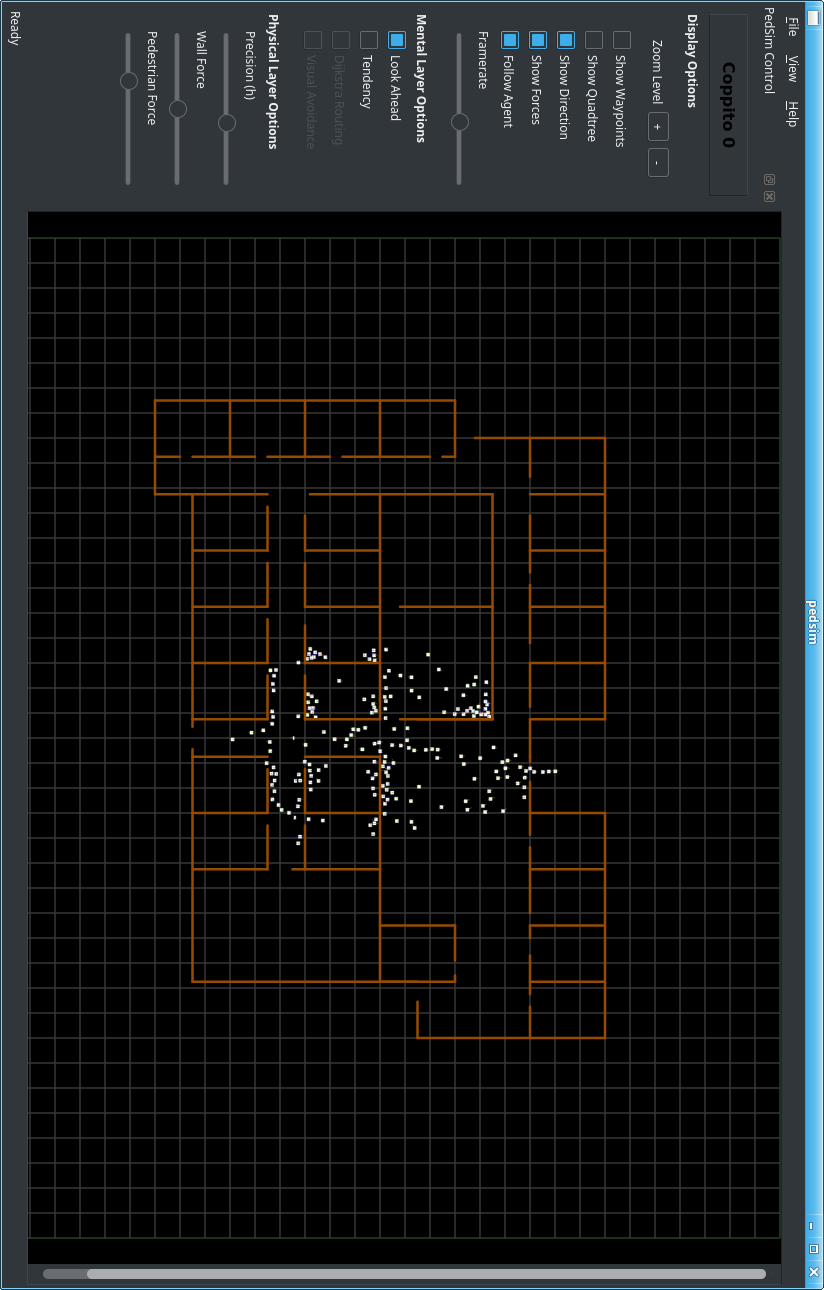
\includegraphics[scale=0.6]{implementation/clutter.png}
	\caption{Agent Cluster Formation in Coppito 0 Building}
  \label{clutter}
\end{figure}

The work also involves in expanding the capabilities of the existing PedSim simulation tool to include the new topology and the also to incorporate the algorithm and also further extended developed from the aforementioned paper and perform a real time analysis between micro and macro agents with the following criteria:

\begin{itemize}
  \item specifying the cells by social distances
  \item respecting the area capacity and doors capacities constraints
  \item setting the speed accordingly for various groups
  \item simulating social attachment among some agents 
\end{itemize}

As it is evident from the above constraints, the goal of this algorithm and this simulation is to make exit strategies as realistic as possible. By grouping certain agents together for instance, we can achieve realistic movement of participating agents, as in reality, people usually move in groups. families, friends etc. Furthermore, congestion is a big part of the evacuation scenario, as it is congestion that determines how fast or efficient the evacuation of agents occur and also how it would take to move groups of people. With groups of people clumped together, the next most natural constraint would be to assign varying speeds as not all agents and not all groups of agents travel with the same speed across the topology of the building. There is also one other constraint which determines the cell capacity, which determines how spaced out and occupied agents are in a room, a hall or a passageway. This also help determine how many can get through a single doorway in order to transition from one passageway to another. This of course leads to previously mentioned issue of congestion. 

All these constraints are hence taken into account as the simulation is performed in order to clock and test for the performance time and efficiency of the algorithm used for micro and macro model simulation.

\section{Thesis Outline}
\label{sec:intro:Thesis Outline}

The structure of the thesis is formulated as follows: chapter 2 provides a detailed literature and background work pertaining to the area of agent based simulation models and exit strategies. Chapter 3 focuses on the implementation details of the algorithm and specific scenario details that are incorporated in order to extend the algorithm in order to adapt it to a more realistic setting and also technical details regarding the PedSim simulation environment. Chapter 4 presents the results of the comparisons of the optimized(realistic) algorithm between the macro and micro agent simulation setting and to chart out the various performance metrics that are obtained. Chapter 5 attempts to draw conclusions based on the obtained performance metrics and also present the future work related to the aforementioned. This thesis also provides a technical appendix for reference for the simulation of various micro and macro agent scenarios within the environment of PedSim.

\chapter{Related Work\label{ch:pastwork}}

In this section the background literature and the work related to agent based simulation is dicussed. 

% include other files for sections of this chapter. These use the 'input' command since each section within a chapter should not start a new page.
% If you want to swap the order of sections, it is as simple as reversing the order you include them. 
\section{Pre-Modern Disaster Preparedness, Management and Relief Techniques}
\label{sec:pastwork:Pre-Modern Disaster Preparedness, Management and Relief Techniques}

Although disasters have existed throughout the history of the universe for all living organisms, human beings are perhaps the only one to be affected on a massive scale as a collective group as we are vulnerable and weak compared to other animals that live and co-exist with us. Hence human beings have taken many steps over the years fortifying and defending ourselves as best as we can through the various buildings and escape routes we design. The early inhabitants of mankind were not idle and did not become easy victims. There is historical evidence that the early man took various measures in order to cope with, reduce and mitigate risks. The mere fact that they chose to inhabit caves are a testament to this theory \cite{ref6}.

The ancient man also used other natural techniques for disaster preparedness. One of the prominent ones include the observation of animals since they are very perceptive to natural disasters, animal behavior can and has been used for the better part of the millenia to predict the onset of a natural disaster such as floods, earthquakes etc. One of the earliest works to be done in this field involves in the observation of the behavior of fish, specifically the catfish, as they were found to exhibit a definitive behavior in advance of the occurence of an earthquake \cite{ref7}. Other experiments and observations pertaining to such natural responses include the obeservation of ground electric field effects on behavior of Albino rats, Mongolian gerbils (sand rats), hair-footed Djungarian hamsters, guinea pigs, and red sparrows \cite{ref8}. A summary of such animal behavior and work is presented by Neeti Bhargava et. al. \cite{ref9}.

To combat various natural disasters that affect us, mankind has tried for over a millenia to improve and adapt buildings, and entire cities to cope during the time of a catatrosphe. There are two broad categories to the mitigation of these disasters that have been long employed \cite{ref10}:

\begin{itemize}
  \item structural based mitigation
  \item non-structural based mitigation
\end{itemize} 

Since my work pertains to indoor simulation and evacuation management, the discussion for non-structural mitigation forms here is considered unnecessary and beyond the scope of this thesis. Structural mitigation involves the presence of a building or a man-made mechanical or technological adaptations performed to reduce hazards and mitigate risks. The following sub-section expands more on the more modern techniques that have been developed over the course of the modern era and their implications. Although better and state of the art systems have been developed over the years, these systems have complications of their own. Failure of the perfect working of an evacuation system leads to the possible death of all the agents who are in need of evacuation. 

\section{Routing Algorithms and IoT Based Evacuation Management}
\label{sec:pastwork:Routing Algorithms and IoT Based Evacuation Management}

Routing algorithms and maze solving algorithms have especially been applied to the structural domains for the real time analysis of shortest paths and obstacle avoidance by both machine and human agents since the time the earliest shortest paths algorithms were developed. The development of the shortest path algorithm by Dijkstra in 1956, especially has seen a plethora of applications in various fields. As one can guess most of its applications have been catered to graph based problems and obstacle avoidance. Shortest paths exit strategy formation approach is a good way to analyse a safe egress as it provides obstacle avoidance as well. How can it successfully be applied to a real disaster scenario? Before the advancements were made to IoT based infrastructure, maze solving algorithms were used to successfully analyze a safe egress. 

IoT and computation systems have brought about a tremendous potential to perceive the environment and then form the necessary strategies that are required to safely escort the human agents to a safe exit point during the time of disaster. Modern evacuation systems have sensors in place to allow for better perception of the world during a disaster scenario. For instance the work by Kobes et al. determined that during fire related disaster scenarios, 56.3\% of the participating agents were able to determine the exit points based on the exit signs when there was no smoke present whilst 81.8\% was able to identify exit points only based on the exit signs when their vision was imparied due to smoke \cite{ref11}. Based on such data for instance, it greatly enhances our need to analyse the fastest and shortest egress path so that all human agents in the vicinity can get to the exit points. The shortest path algorithm - Dijkstra's algorithm is currently used as a great tool to provide the shortest exit points as it is demonstrated in the work by Jehyun Cho \cite{ref12}. This research pertains to the dynamic analysis of a shortest path algorithm based on information obtained from the sensors and the smart infrastructure.  

In order to address the issue of agent(s) and infrastructure mapping during a disaster event, smart sensors are placed all through the infrastructure in order to perceive the environment and the surrounding structures in order to analyze a safe egress. Motion detectors for instance are used to understand how many people are still trapped inside the building during a catastrophe. One example of using IoT technologies is proposed by Prasad Annadata et al. using multiple WIFI channels and the aforementioned motion detectors \cite{ref13}. Based on the statistics gathered heuristic solutions are proposed in order to detect the number of personnel inside the infrastructure as well as perceive the environment. 

Although the proposed methods and techniques are helpful in determining the shortest path to an exit point, they rarely can be used in a realistic scenario due to its simplistic nature. A real world scenario is more complex due the social dynamics of people. Such complexities are better understood while simulating agents in real and static simulations and then performing an analysis based on the observed stats. Such is achieveed through this thesis.

Existing literature on surveying personnel and the surrounding infrastructure for assistance based support for immediate first responders include the work done by Palmieri et al., who proposes a hybrid cloud architecture to manage and store the necessary required resources to command and control activities during emergencies \cite{ref14}. However the work done by H. Muccini et al. \cite{ref5} aims to improve this work by adapting geolocation of first responders to track people during a disaster for evacuation. Furthermore W.Choi et al. \cite{ref15} proposes to model building evacuation by dynamic flow maximization and by considering variable capacities on some arcs as a function of flows in incident arcs. For the purposes of modeling our topology we have used a similar arc based geometry for determining the topological capacity of a particular cell into which the entire infrastructure is divided into. Chen et al. \cite{ref16} in addition to the above, proposes a flow control algorithm that calculates evacuation paths depending on building plan and total number of
evacuees. Computation in this case aims at minimizing total evacuation time and assigning an optimal number of evacuees to each evacuation path. However [5] provides a robust solution by architecting an IoT system to monitor and update dynamically the topology of the environment.

Another important aspect that remains unaddressed is that in real disaster scenarios, over crowding and congestion of certain pathways and exit points are bound to occur frequently. The issue of congestion is serious and perilous and is arguably pointed out by a case study performed by John El Khoury \cite{ref17} and analyses the dangers due to high traffic intensity during a disaster event. Although the analysis is performed on a wide scale city range, the implications of congestion and other such constraints are just applicant to a much smaller scale infrastructure. To dynamically reallocate personnel to routes that are not just shortest paths but optimal paths is what we try to achieve through these simulations and added constraints. The work done by Antoine Desmet et al. \cite{ref18} addresses the congestion issue by a "self adaptation" algorithm much inspired by the computer network routing algorithm - The Cognitive Packet routing algorithm by E. Gelenbe \cite{ref19}. A robust evacuation with optimized routing solution proposed by H.Muccini et al. [5] are as follows:

\begin{itemize}
  \item Optimal solutions that can be continuously updated, so evacuation guidelines can be adjusted according to visitors position that evolve over time.
  \item Paths that become suddenly unfeasible can automatically be discarded by the system.
  \item The model can be incorporated into a mobile app supporting emergency units to evacuate closed or open spaces.
\end{itemize} 

The aforementioned algorithm although is complete and optimized, additional dynamic and realistic constraints are yet to be added during an evacuation scenario. The constraints are 4 fold as mentioned in the introduction section. Over the course of chapter 3, the details of the algorithm is explained and how these constraints provide a more optimized simulation scenario since it considers congestion, grouping, varying age and speeds in addition. 

\section{Simulation Tools and Constraints}
\label{sec:pastwork:Simulation Tool and Constraints}

In order to accomodate for accurate results and model precise human behavior, agent based modeling and simulations have become increasingly popular as computational expenses became cheaper and ever more accessible. In addition to developing state of the art routing algorithms and other obstacle avoidance mechanisms, it was also absolutely important to understand human behavior and the complex decisions that agents make during a catastrophic event. To understand the implications of human behavior and complex real-time decision making and other realistic constraints, this thesis presents various scenarios that are depicted in a small to a large scale microscopic agent based fashion in hopes to draw out some interesting conclusions based on the obtained results. One such example of the kind of work that we are hoping to perform is the impairment of certain agents based on the circumstances that are met with in real time during the disaster event. The work presented by Selain Kasereka et al. \cite{ref20} offers a unique insight into modeling agents for a fire disaster and simulating the case for some interesting results. It should be mentioned that the case presented in the current thesis however is modeled for a generic scenario. In the work presented, the smoke and fire can affect the agent, thus reducing their potency and their ability to escape from danger. This damage to potency can be essentially translated to a reduced movement speed and a severe impairment to their cognitive ability to perform real time decisions. 

Another really interesting thing to point out is about psychology and human behavior during ground zero scenarios. Human panic and confusion is generally a chaotic element that must certainly be infused into such simulations as they provide further insight into human behavior and particularly decisions that lead to increase or the decrease in congestion. Based on certain decisions and paths, it may cause discomfort or physical pain to some and many agents within the promixity of such an incident. Ashutosh Trivedi et al. \cite{ref21} provides a detailed analysis and where different strategies are evaluated and the corresponding evacuation time and physical discomfort caused to the agents are observed. He justifies the effect of social forces based on cohesion which, in my thesis, is also considered whilst perfoming simulation for microscopic agents. Our work revolves very closely the work done by A. Trivedi et al. as it also deals with social forces, panic and other realistic constraints. Through this thesis, experimental analysis for these sophisticated constraints are performed for both macro and micro agents in hopes for better understanding and formulating a safe egress for the agents.

Simulation tools have been used since the inception of computers and computation technology since the early 1970s. Modern simulations for evacuation and relief management includes the simulations of pedastrians and agents within the domains of the inscribed topology, with start and end points. These simulations are then run against various parameters and scenarios thus obtaining various results. Through this thesis the various experiments are simulated within the environment of PedSim, a massive microscopic real time simulator. The in depth analysis of large number agents based simulators are provided by the extensive and comprehensive survey presented in "Agent Based Modelling and Simulation tools: A review of the state-of-art software" by Sameera Abar et al. \cite{ref22}. The survey is based on the following criteria which is presented as follows:

\begin{itemize}
  \item License/Availability
  \item Source Code in which the simulator is written in
  \item Type of Agent based on its interaction and behavior
  \item Coding language or application programming interface(API) for Model Development; Integrated Development Environment(IDE) used
  \item Compiler/Operating System/Implementation Platform
  \item Model Development Effort
  \item Modelling Strength/Simulation Models' Scalability Level
  \item ABMS scope or Application Domain
\end{itemize} 

From the extensive survey provided, it was easily inferred that PedSim, pedastrian microscopic simulator was the best suited for testing the various scenarios as it could support both micro and macro based agent modelling scenarios and grouping. It must also be mentioned that the tool is entirely written in C++, extremely light-weight and highly scalable. It also works well on development platforms and can be compliled easily on all operating systems. Its simple and easy to use, as complex simulations can be run for massive number of agents and the results can be visualized in real time. For all these reasons I have decided to use PedSim exclusively as my test bed tool whilst modelling such scenarios. 

In the following section the scenario and the implementation details of my work will be discussed.


% 
\chapter{Usage\label{ch:usage}}

To start, in your main .tex file, use this class as your main documentclass instead of `report' or `book'. For example:
\begin{quote}
$\backslash documentclass[12pt,lot, lof]\{puthesis\}$
\end{quote}

In this example, we setup our document to use the PU Thesis style, with 12pt font for body text, and to include a List of Tables and List of Figures in the front matter. You could instead set an 11 point or 10 point font by changing the first option. You can also add `los' to include a list of symbols.

To use single spacing, add the option `singlespace'. This is a special option for the \texttt{puthesis} documentclass, which sets single spacing for both the front matter and for the document itself. Additional parameters should be set in your main .tex file, and are described in detail in Section~\ref{sec:usage:options}.

The template itself declares two other options, to be set immediately after the \texttt{documentclass} command. First is `printmode', declared with the command:
\begin{quote}
$\backslash newcommand\{\backslash printmode\}\{\}$
\end{quote}
This command, used later in the thesis.tex file, turns off the \texttt{hyperref} package and all internal links in the PDF file. This removes any colored links and highlighting that would not be appropriate in a printed and bound thesis. Instead the \texttt{url} package is loaded, so that \\url commands in your document will continue to work and urls will break properly across multiple lines.

When `printmode' is not specified, the hyperref package is included. It creates colored links for citations, footnotes, and internal references, which can be used to navigate the PDF document more easily. It also adds bookmarks to the PDF file, mirroring the table of contents. By default, it is set to use colored links. For the PDF file that you will submit electronically to ProQuest, this may not be desirable since some copies may be printed, while others will be used electronically. Thus another option, `proquestmode', is defined that keeps hyperref but disables colored links:
\begin{quote}
$\backslash newcommand\{\backslash proquestmode\}\{\}$
\end{quote}
This mode has no effect when used in combination with `printmode'. 


\section{Options}
\label{sec:usage:options}

In this section, we describe the options you can set when using this thesis class.
\tablespacing
% tablespacing is defined by the class to set single spacing for the long table when in doublespacing mode. If the singlespace option is set, this command has no effect.

\begin{longtable}{p{0.3\linewidth} p{0.6\linewidth}}

  % First page heading
  \caption[Options Provided by the PUthesis Class]{List of options for the puthesis document class and template} \label{tab:usage:options}\\
  \toprule
  \textbf{Option} & \textbf{Description} \\
  \midrule
  \endfirsthead

  % Future page heading
  \caption[]{(continued)}\\
  \toprule
  \textbf{Option} & \textbf{Description} \\
  \midrule
  \endhead

  % Page footer
  \midrule
  \multicolumn{2}{r}{(Continued on next page)}\\
  \endfoot

  % Last page footer
  \bottomrule
  \endlastfoot

  12pt &
  Specify the font size for body text as a parameter to \texttt{documentclass}. The Mudd Library requirements~\cite{muddthesis2009} state that 12pt is preferred for serif fonts (e.g., Times New Roman) and 10pt for sans-serif fonts (e.g., Arial).
  \\

  letterpaper &
  If your document is coming out in a4paper, your LaTeX defaults may be wrong. Set this option as a parameter to \texttt{documentclass} to have the correct 8.5"x11" paper size.
  \\

  lot &
  Set this option as a parameter to \texttt{documentclass} to insert a List of Tables after the Table of Contents.
  \\


  lof &
  Set this option as a parameter to \texttt{documentclass} to insert a List of Figures after the Table of Contents and the List of Figures.
  \\

  los &
  Set this option as a parameter to \texttt{documentclass} to insert a List of Symbols after the Table of Contents and the other lists.
  \\

  singlespace &
  Set this option as a parameter to \texttt{documentclass} to single space your document. Double spacing is the default otherwise, and is required for the electronic copy you submit to ProQuest. Single spacing is permitted for the printed and bound copies for Mudd Library.
  \\
  
  draft &
  Set this option as a parameter to \texttt{documentclass} to have \LaTeX mark sections of your document that have formatting errors (e.g., overfull hboxes). 
  \\

  % the cmidrule here spans both columns but is indented slightly on the left and right. 
  \cmidrule[0.1pt](l{0.5em}r{0.5em}){1-2}

  \raggedright
  $\backslash newcommand$ $\{\backslash printmode\}\{\}$ &
  Insert this command after the \texttt{documentclass} command to turn off the hyperref package to produce a PDF suitable for printing.
  \\

  \raggedright
  $\backslash newcommand$ $\{\backslash proquestmode\}\{\}$  &
  Insert this command after the \texttt{documentclass} command to turn off the `colorlinks' option to the hyperref package. Links in the pdf document will then be outlined in color instead of having the text itself be colored. This is more suitable when the PDF may be viewed online or printed by the reader.
  \\

  $\backslash makefrontmatter$ &
  Insert this command after the \texttt{$\backslash begin\{document\}$} command, but before including your chapters to insert the Table of Contents and other front matter.
  \\
  
  \cmidrule[0.1pt](l{0.5em}r{0.5em}){1-2}

  $\backslash title$ &
  Set the title of your dissertation. Used on the title page and in the PDF properties.
  \\

  $\backslash submitted$ &
  Set the submission date of your dissertation. Used on the title page. This should be the month and year when your degree will be conferred, generally only January, April, June, September, or November. Check the Mudd Library rules~\cite{mudd2009} for the appropriate deadlines.
  \\

  $\backslash copyrightyear$ &
  Set the submission year of your dissertation. Used on the copyright page.
  \\

  $\backslash author$ &
  Your full name. Used on the title page, copyright page, and the PDF properties. \\

  $\backslash adviser$ &
  Your adviser's full name. Used on the title page. \\

  $\backslash departmentprefix$ &
  The wording that precedes your department or program name. Used on the title page. The default is ``Department of'', since most people list their department and can leave this out (e.g., Department of Electrical Engineering), however if yours is a program, set $\backslash departmentprefix\{Program in\}$ \\

  $\backslash department$ &
  The name of your department or program. Used on the title page. \\

  \cmidrule[0.1pt](l{0.5em}r{0.5em}){1-2}
  
  \raggedright  
  $\backslash renewcommand$ $\{\backslash maketitlepage\}\{\}$ &
  Disable the insertion of the title page in the front matter. This is useful for early drafts of your dissertation. \\

  \raggedright  % full justification places the * in an awkward place
  $\backslash renewcommand*\{\backslash makecopyrightpage\}\{\}$ &
  Disable the insertion of the copyright page in the front matter. This is useful for early drafts of your dissertation. \\

  \raggedright 
  $\backslash renewcommand*\{\backslash makeabstract\}\{\}$ &
  Disable the insertion of the abstract in the front matter. This is useful for early drafts of your dissertation. \\

\end{longtable}
\bodyspacing
% bodyspacing restores double spacing or single spacing after the table

% need blank space after \bodyspacing

I've seen other people print their dissertations using $\backslash pagestyle\{headings\}$, which places running headings on the top of each page with the chapter number, chapter name, and page number. This documentclass is not currently compatible with this option -- the margins are setup to be correct with page numbers in the footer, placing them 3/4" from the edge of the paper, as required. If you wish to use headings, you will need to adjust the margins accordingly.
 




% 
\chapter{Conclusion\label{ch:conclusion}}

From the presented scenario and cases, it is quite evidently evaluated that micro agent simulation, optimized with the applied realistic constraints presents the most realistic approach to evacuation compared to the other cases. Based on this objective presentation, we can design topologies and evacuation systems that are better suited to accommodate the required crowd of pedastrians. Through this thesis, it is also shown how adding even a small constraint to the simulation can severely alter the overall evacuation time of the agents. The nature of these constraints and how they affect the overall evacuation performance of the agents helps us to be better prepared in the likelihood of an actual disaster event.    

The present work employs a software architecture that helps improve and optimise the evacuation time which is very crucial in the case of an emergency. From the topology data obtained, it is pipelined into PedSim simulation environment. Once this data and the distribution of people is fed in to the system, the algorithm for evacuation provides a generic initial pathway to the agents and as time progresses, provides an alternate/optimal paths for various agents and suggest the paths suitable to each individual. This is achieved by dividing the floor plan first into blocks and subsequently into number of cells. The cells may have different orientations-horizontal and vertical. The paths are not allowed to cut through walls. The walls can be in any place even inside the rooms. Safe passage through the doors are then computed which connects to those to safe areas can then be computed. This modular nature of the algorithm makes it easy to scale the versions for future architecture and add more constraints by add-on modules. The simulation tool allows itself to upgraded to more generic pathing algorithm as well.  The following are the advantages that are due to the present simulation tool and the employed algorithm:

\begin{itemize}
\item All possible trajectories are computed.
\item The optimal paths to safe areas are selected from the same.
\item Regulates the flow as per the constraints to reduce congestions.
\item Erratic and random  motions are reduced.
\item Evacuation plan is made available to one and all.
\item Simulation is carried out in design time, although monitoring the status of evacuation is done in real time.
\item Can easily be integrated to IoT based framework.
\item Optimal evacuation procedure model can be evolved from the resulting simulations.
\end{itemize}

 % Conclusion
\section{Future Work}

This work can be extended to non-standard buildings with additional constraints in future. The internet of things (IoT) helps in locating the number of persons in each block and their location (cell numbers) which can then be dynamically fed in to the simulation tool for optimisation in real time. When such data can be obtained, the simulation can then be shifted from design time to a real time egress path evaluation. 


 
 % Future work

% \appendix % all chapters following will be labeled as appendices
% \chapter{Scenario Definition\label{ch:Scenario Definition}}

This section is used to provide a brief technical description of the implementation details that are involved whilst defining a scenario for the simulation of pedastrian agents within the PedSim environment. The library modules are written entirely in C++ whilst the topology description is described within a .xml file. The simulation tool parses the xml file and graphically projects the topology onto the simulation environment for visual reference.
The agent properties are also defined in the xml file such as their base speed, spawn location, total number of agents etc.

The section below provides an example of writing a topology description in the .xml file.

\section{Defining Topology}

The code snippet presented below depicts an example of defining the outline of the building, which was the topology used to run the simulations in. The dimensions of the building are strictly modeled according to the figure \ref{Coppito0 layout}. The dimensions have been scaled up to 5 times in order to suit the PedSim environment. A typical obstacle/wall description is defined as follows:
\\

\begin{lstlisting}[language=xml]
  <!-- Outer Walls -->
  
  <!-- TOP SIDE -->
  <obstacle x1="-120" y1="-90" x2="-7.5" y2="-90" />
  <obstacle x1="-7.5" y1="-90" x2="-7.5" y2="-60" />
  <obstacle x1="-7.5" y1="-60" x2="7.5" y2="-60" />
  <obstacle x1="7.5" y1="-60" x2="9.5" y2="-60" />
  <obstacle x1="17.5" y1="-60" x2="30" y2="-60" />
  <obstacle x1="30" y1="-60" x2="30" y2="-90" />
  <obstacle x1="30" y1="-90" x2="120" y2="-90" />

  <!-- RIGHT SIDE -->
  <obstacle x1="120" y1="-90" x2="120" y2="-15" />
  <obstacle x1="120" y1="-15" x2="105.5" y2="-15" />
  <obstacle x1="97.5" y1="-15" x2="97.5" y2="75" />

  <!-- BOTTOM SIDE -->
  <obstacle x1="97.5" y1="75" x2="7.5" y2="75" />
  <obstacle x1="7.5" y1="75" x2="4.5" y2="75" />
  <obstacle x1="-4.5" y1="75" x2="-7.5" y2="75" />
  <obstacle x1="-7.5" y1="75" x2="-97.5" y2="75" />
  <obstacle x1="-97.5" y1="75" x2="-97.5" y2="90" />
  <obstacle x1="-97.5" y1="90" x2="-135" y2="90" />


  <!-- LEFT SIDE -->
  <obstacle x1="-135" y1="90" x2="-135" y2="-30" />
  <obstacle x1="-135" y1="-30" x2="-112.5" y2="-30" />
  <obstacle x1="-120" y1="-38" x2="-120" y2="-90" />

\end{lstlisting}

From the above code snippet, the x and y pair points are given for drawing straight lines.
Partial and full agent pathing can be provided for the agents in order for them to start moving towards exit points during an emergency scenario.

\begin{lstlisting}[language=xml]

  <!-- waypoints are defined before agents  -->
  
  <waypoint id="w1" x="-75.0" y="-10" r="2" />
  <waypoint id="w2" x="-61" y="-3" r="2" />
  <waypoint id="w3" x="-50" y="-3" r="2" />
  <waypoint id="w4" x="-40" y="-3" r="2" />
  <waypoint id="w5" x="-30" y="-3" r="2" />
  <waypoint id="w6" x="-7.5" y="-3" r="2" />
  <waypoint id="w7" x="0" y="0" r="2" />
  <waypoint id="w8" x="0" y="30" r="2" />
  <waypoint id="w9" x="0" y="40" r="2" />
  <waypoint id="w10" x="0" y="50" r="2" />
  <waypoint id="w11" x="0" y="60" r="2" />
  <waypoint id="w12" x="0" y="70" r="2" />
  <waypoint id="w13" x="0" y="90" r="2" />

  \end{lstlisting}

The waypoint definition has coordianates x, y and radius r. The .xml file was written by referring the official documentation as provided in \cite{ref26}. Sample scenarios and tutorials regarding the same are also provided in the same documentation.

The final step in completing the scenario description is to include the agent properties. Given below is a sample agent definition in xml:

\begin{lstlisting}[language=xml]
  <agent x="30" y="-30" n="10" dx="50" dy="50">
  
  \end{lstlisting}

Where,
\begin{itemize}
\item $n$ is the number of agents.
\item $x$ and $y$ are the spawn location of the agents within the topography of the environment.
  \item dx and dy are used to determine the spread of the agents spawned. Agents are distributed evenly according to $x - dx$ and $x + dx$ and correspondingly along $y - dy$ and $y + dy$.
  \end{itemize}

Varying $n$ allows for defining the number of agents in a given group. This is particularly useful for the group simulation scenarios. In order to perform micro agent simulations, the $n$ is typically valued as 1. To summarize the agent definition, waypoints for the agents are defined in order to provide a more definitive pathing for the agents based on the spawn locations.

For a micro agent simulation, the agent definition will be as follows:
\\

\begin{lstlisting}[language=xml]
  
  <agent x="30" y="-30" n="1" dx="50" dy="60">
  <addwaypoint id="wu" />
  <addwaypoint id="wd" />
  <addwaypoint id="wz" />
  </agent> 
  <agent x="30" y="-30" n="1" dx="25" dy="30">
  <addwaypoint id="wu" />
  <addwaypoint id="wd" />
  <addwaypoint id="wz" />
  </agent> 
  <agent x="30" y="-30" n="1" dx="94" dy="100">
  <addwaypoint id="wu" />
  <addwaypoint id="wd" />
  <addwaypoint id="wz" />
  </agent> 
  <agent x="30" y="-30" n="1" dx="107" dy="112">
  <addwaypoint id="wu" />
  <addwaypoint id="wd" />
  <addwaypoint id="wz" />
  </agent>
    
\end{lstlisting}

Once the scenario to be modeled is described in the .xml file as given in the above code snippets, the file is then parsed by the PedSim library modules. Once the data is parsed from the .xml file, the agents are spawned according to the provided definitions and then PedSim proceeds to simulate the agents along the general waypoints as configured from the previous file.

The PedSim library modules are modified and extended in order to simulate the agents according to the algorithm present in \cite{ref5}. The technical details and description are provided in brief in the next section.
 

% \chapter{Printing and Binding\label{ch:printing}}

\section{Printing}

For the library copies of your dissertation, you must use archival quality printing and binding. This means acid-free paper, containing at least 25\% cotton fiber. Triangle Repocenter on Nassau Street in Princeton offers both 25\% cotton paper and 100\% cotton paper. Most people choose the 25\% cotton paper, and this is generally recommended by the binders. The 100\% copy paper is somewhat thicker and the extra expense is unnecessary. 

Triangle offers online submission of your printing and binding order at: \url{http://triangleprinceton.com/collegiatebinding/thesis/}. If you request binding from them, they will deliver the paper copies to Smith-Shattuck Bookbinding for you and allow you to pick up the completed copies at their store on Nassau Street. The whole process takes 2-3 business days, but check with them in advance during the busy thesis-printing season in April and May. 

Currently, your printed and bound dissertation copies can be single spaced. Only the electronic copy submitted to ProQuest must be double spaced. All copies must be printed single-sided, with specific margins. 

\section{Binding}

An archival-quality sewn binding is required for the library copies of your dissertation. Smith-Shattuck Bookbinding is highly recommended, and is used by most students. Triangle Repocenter will send your copies there for you, greatly simplifying the process, but you can call Smith-Shattuck with special requests. 

The ``library standard'' sewn binding is sufficient for the copies to be sent to Mudd Library. It uses a black buckram cloth cover, which is the most popular option. For extra copies for yourself and your family members, you can choose ``buckram roundback binding'', which adds decorative lines on the spine, and printing of the title and author on the front cover. For a small additional fee, you can include the Princeton University shield on the front cover and a ribbon bookmark. Leather covers are also available. See Smith-Shattuck's website for more details at: \url{http://www.thesisbookbinding.com/}. 


% Make the bibliography single spaced
\singlespacing
\bibliographystyle{plain}

% add the Bibliography to the Table of Contents
\cleardoublepage
\ifdefined\phantomsection
  \phantomsection  % makes hyperref recognize this section properly for pdf link
\else
\fi
\addcontentsline{toc}{chapter}{Bibliography}

% include your .bib file
\bibliography{thesis}

\end{document}

